\documentclass[letterpaper,10pt]{article}
\usepackage{listings}
\usepackage{color}
\usepackage{algorithm2e}
\usepackage{graphicx}
\usepackage{epstopdf}
\usepackage{multirow}
\usepackage[margin=1.0in]{geometry}
\usepackage{amsmath,amsthm,amssymb}
 
\definecolor{dkgreen}{rgb}{0,0.6,0}
\definecolor{gray}{rgb}{0.5,0.5,0.5}
\definecolor{mauve}{rgb}{0.58,0,0.82}
 
\lstset{ %
  language=C++,                % the language of the code
  basicstyle=\footnotesize,           % the size of the fonts that are used for the code
  numbers=left,                   % where to put the line-numbers
  numberstyle=\tiny\color{gray},  % the style that is used for the line-numbers
  stepnumber=1,                   % the step between two line-numbers. If it's 1, each line 
                                  % will be numbered
  numbersep=5pt,                  % how far the line-numbers are from the code
  backgroundcolor=\color{white},      % choose the background color. You must add \usepackage{color}
  showspaces=false,               % show spaces adding particular underscores
  showstringspaces=false,         % underline spaces within strings
  showtabs=false,                 % show tabs within strings adding particular underscores
  frame=single,                   % adds a frame around the code
  rulecolor=\color{black},        % if not set, the frame-color may be changed on line-breaks within not-black text (e.g. commens (green here))
  tabsize=2,                      % sets default tabsize to 2 spaces
  captionpos=b,                   % sets the caption-position to bottom
  breaklines=true,                % sets automatic line breaking
  breakatwhitespace=false,        % sets if automatic breaks should only happen at whitespace
  title=\lstname,                   % show the filename of files included with \lstinputlisting;
                                  % also try caption instead of title
  keywordstyle=\color{blue},          % keyword style
  commentstyle=\color{dkgreen},       % comment style
  stringstyle=\color{mauve},         % string literal style
  escapeinside={\%*}{*)},            % if you want to add LaTeX within your code
  morekeywords={*,...}               % if you want to add more keywords to the set
}

% Title Page
\title{Assignment 3: Linear Programming project}
\author{Francis Vo, Soo-Hyun Yoo}

\setlength{\parindent}{0cm}
\setlength{\parskip}{1em}

\begin{document}
	\maketitle

	\section{Problem 1: mmmm \dots pork}

	\subsection{Mathematical Model}
		\subsubsection{Objective Function}
			%max\\
			%$8 * ham\_f + 12 * ham\_r + 11 * ham\_o + $\\
			%$4 * bellies\_f + 12 * bellies\_r + 7 * bellies\_o + $\\
			%$4 * picnics\_f + 13 * picnics\_r + 9 * picnics\_o$
			\begin{align*}
				\text{max} ( & 8\cdot\text{ham}_f + 12\cdot\text{ham}_r + 11\cdot\text{ham}_o + \\
							 & 4\cdot\text{bellies}_f + 12\cdot\text{bellies}_r + 7\cdot\text{bellies}_o + \\
							 & 4\cdot\text{picnics}_f + 13\cdot\text{picnics}_r + 9\cdot\text{picnics}_o )
			\end{align*}

		\subsubsection{Constraints}
			\begin{align*}
				\text{ham}_f + \text{ham}_r + \text{ham}_o             &\le 480 \\
				\text{bellies}_f + \text{bellies}_r + \text{bellies}_o &\le 400 \\
				\text{picnics}_f + \text{picnics}_r + \text{picnics}_o &\le 230 \\
				\text{ham}_r + \text{bellies}_r + \text{picnics}_r     &\le 420 \\
				\text{ham}_o + \text{bellies}_o + \text{picnics}_o     &\le 250
			\end{align*}


	\subsection{Standard Form}
		\subsubsection{Objective Function}
			\begin{align*}
				\text{max} ( & 8\cdot\text{ham}_f + 12\cdot\text{ham}_r + 11\cdot\text{ham}_o + \\
							 & 4\cdot\text{bellies}_f + 12\cdot\text{bellies}_r + 7\cdot\text{bellies}_o + \\
							 & 4\cdot\text{picnics}_f + 13\cdot\text{picnics}_r + 9\cdot\text{picnics}_o )
			\end{align*}

		\subsubsection{Constraints} 
			%$\text{ham}_f + \text{ham}_r + \text{ham}_o + \text{ham}_remain = 480$\\
			%$\text{bellies}_f + \text{bellies}_r + \text{bellies}_o + \text{bellies}_remain = 400$\\
			%$\text{picnics}_f + \text{picnics}_r + \text{picnics}_o + \text{picnics}_remain = 230$\\
			%$\text{ham}_r + \text{bellies}_r + \text{picnics}_r + smoke\_reg = 420$\\
			%$\text{ham}_o + \text{bellies}_o + \text{picnics}_o + smoke\_over = 250$\\
			%$\text{ham}_remain, \text{bellies}_remain, \text{picnics}_remain, smoke\_reg, smoke\_over \ge 0$\\

			% Francis's try at making it look nice, redone by Soo-Hyun -- don't use tables!
			\begin{align*}
				\text{ham}_f + \text{ham}_r + \text{ham}_o + \text{ham}_\text{remain}                 &= 480 \\
				\text{bellies}_f + \text{bellies}_r + \text{bellies}_o + \text{bellies}_\text{remain} &= 400 \\
				\text{picnics}_f + \text{picnics}_r + \text{picnics}_o + \text{picnics}_\text{remain} &= 230 \\
				\text{ham}_r + \text{bellies}_r + \text{picnics}_r + \text{smoke}_\text{reg}   &= 420 \\
				\text{ham}_o + \text{bellies}_o + \text{picnics}_o + \text{smoke}_\text{over}  &= 250 \\
				\text{ham}_\text{remain}, \; \text{bellies}_\text{remain}, \; \text{picnics}_\text{remain}, \; \text{smoke}_\text{reg}, \; \text{smoke}_\text{over} &\ge 0
			\end{align*}


	\subsection{Matrix Form}
	We wish to find max($cx$), where
	
	\[
		c =
		\begin{pmatrix}
			8 & 14 & 11 & 4 & 12 & 7 & 4 & 13 & 9
		\end{pmatrix},
	\]

	and

	\[
		x =
		\begin{pmatrix}
			\text{ham}_f \\
			\text{ham}_r \\
			\text{ham}_o \\
			\text{bellies}_f \\
			\text{bellies}_r \\
			\text{bellies}_o \\
			\text{picnics}_f \\
			\text{picnics}_r \\
			\text{picnics}_o
		\end{pmatrix}
		\geq 0.
	\]

	Also,

	\[
		\begin{pmatrix}
			1 & 1 & 1 & 0 & 0 & 0 & 0 & 0 & 0 \\
			0 & 0 & 0 & 1 & 1 & 1 & 0 & 0 & 0 \\
			0 & 0 & 0 & 0 & 0 & 0 & 1 & 1 & 1 \\
			0 & 1 & 0 & 0 & 1 & 0 & 0 & 1 & 0 \\
			0 & 0 & 1 & 0 & 0 & 1 & 0 & 0 & 1
		\end{pmatrix}
		\begin{pmatrix}
			\text{ham}_f \\
			\text{ham}_r \\
			\text{ham}_o \\
			\text{bellies}_f \\
			\text{bellies}_r \\
			\text{bellies}_o \\
			\text{picnics}_f \\
			\text{picnics}_r \\
			\text{picnics}_o
		\end{pmatrix}
		\le
		\begin{pmatrix}
			480 \\
			400 \\
			230 \\
			420 \\
			250
		\end{pmatrix}.
	\]


	\newpage
	\subsection{Solution}
		Total net profit: \$10,910 \\

		\begin{tabular}{|l|ccc|} \hline
			& fresh & smoked on regular time & smoked on overtime \\ \hline
			hams    & 440 & 0   & 40 \\
			bellies & 0   & 400 & 0 \\
			picnics & 0   & 20  & 210 \\ \hline
		\end{tabular}
		%\lstinputlisting{pork.sol}

	\subsection{Using an LP-solver}
		We used the GNU Linear Programming Kit to solve this problem. The help page tells us that we should give a model file (provided in the next section) to glpsol, which we do by running: {\tt glpsol -m pork.mod -o pork.sol}.

	\subsection{Code}
		\lstinputlisting{pork.mod}


	\section{Problem 2: least squares isn’t good enough for me}

	\subsection{Mathematical Model}
		\subsubsection{Objective function}
		min($t$)

		\subsubsection{Constraints}
		Given a set of points $(x_1,y_1), (x_2,y_2), \dots, (x_n,y_n)$,

		\begin{align*}
			|x_i - b| &\le t, \text{ and} \\
			|ax_i + by_i - c| &\le t,
		\end{align*}

		for $1 \le i \le n$.


	\subsection{Standard Form}
		\subsubsection{Objective Function}
		min($t$)

		\subsubsection{Constraints}
		Given a set of points $(x_1,y_1), (x_2,y_2), \dots, (x_n,y_n)$,

		\begin{align*}
			x_i - b + v_i = t \\
			x_i - b \ge -t \\
			ax_i + by_i - c + z_i = t \\
			ax_i + by_i - c \ge -t \\
			v_i, z_i \ge 0
		\end{align*}

		for $1 \le i \le n$.


	\subsection{Solution}
		The solution for the specific problem is as follows:
		\[a = -8.8\]
		\[b = 5.5\]
		\[c = 12\]
		This best fit line is shown in Figure~\ref{fig:plot}.

	%\lstinputlisting{bestFit2.sol}


	\subsection{Plot}
		\begin{figure}[!htb]
			\centering
			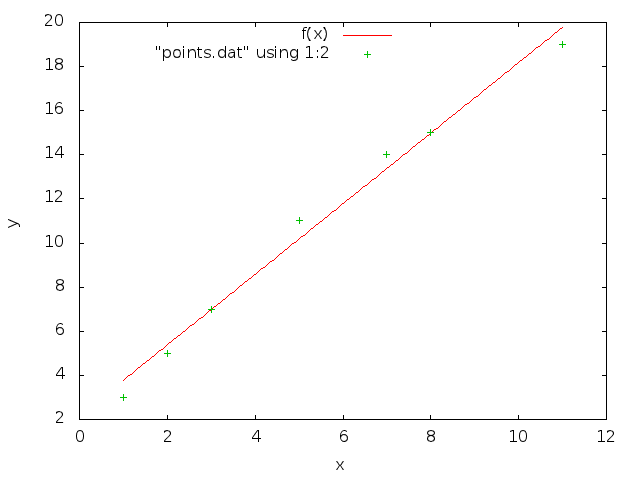
\includegraphics[width=6in]{plot.png}
			\caption{Points and best fit line.}
			\label{fig:plot}
		\end{figure}


	\newpage
	\subsection{Code}
		\lstinputlisting{bestFit.mod}

\end{document}
